\documentclass[12pt]{article}
\usepackage{amsmath}
\usepackage{fullpage}
\usepackage[authoryear,round]{natbib}
\usepackage{lineno}
\usepackage{graphicx} 
\usepackage{setspace}
\doublespacing
\sloppy

\title{Density-dependent selection and the limits of relative fitness}
\author{Jason Bertram $^{1,\ast}$ \\ 
Joanna Masel $^{1}$}

\date{}

\begin{document}

\maketitle

\noindent{}1. Department of Ecology and Evolutionary Biology, University of Arizona, Tucson, AZ 85721.

\noindent{}$\ast$ Corresponding author; e-mail: jbertram@email.arizona.edu.

\bigskip

\textit{Keywords}: Lottery model, competitive Lotka-Volterra, $r$/$K$-selection, interference competition, eco-evo.

\bigskip

\textit{Author contributions}: JB and JM conceptualized the manuscript. JB did the formal analysis. JB wrote the manuscript with review and editing from JM. 

\bigskip

\textit{Running title}: Density-dependence and relative fitness

\bigskip

\textit{Acknowledgments}: We thank Peter Chesson and Joachim Hermisson for many constructive comments on an earlier and quite different version of this manuscript. This work was financially supported by the National Science Foundation (DEB-1348262) and the John Templeton Foundation (60814).

\linenumbers{}
\modulolinenumbers[1]

\newpage{}


\section*{\centering \huge  Density-dependent selection and the limits of relative fitness}

\bigskip

\subsection*{Abstract}

[I'm going to revise this after your next round of comments]
Selection is commonly described by assigning relative fitness values to genotypes. Yet when selection is strong, the ecological view of selection in density-regulated populations seems to be incompatible with constant-density relative fitnesses. Here we analyze the population ecological limits of relative fitness using a novel of density-dependent selection which contains a ``reproductive excess’’. Our model clearly distinguishes between density-dependent selection and changes in density driven by selection. These two effects are confounded in standard models of density-regulated population growth, but both are necessary, in combination with strong selection, for relative fitness to break down in populations close to demographic equilibrium. Remarkably, both effects are not sufficient: we give an example of strong selection on a density-regulating trait subject to density-dependent selection that conforms to the density-independent relative fitness description almost exactly. We reiterate the importance of reproductive excesses in many species, which allows even strong selection to have no effect on density. Our model also offers a possible alternative to relative fitness when the latter is untenable, as is likely the case far from demographic equilibrium. 

\noindent (191 words)

\newpage{}


\section*{Introduction}

There are a variety of different measures of fitness, such as expected lifetime reproductive ratio $R_0$, intrinsic population growth rate $r$, equilibrium population density/carrying capacity (often labeled ``$K$'') \citep{benton_2000}, and invasion fitness \citep{metz_1992}. In addition, ``relative fitness'' is widely used in evolutionary genetics, where the focus is on relative genotypic frequencies \cite[pp. 468]{barton_2007}. The variety of fitness measures is not problematic in itself, but it should be clear how these measures are connected to the processes of birth and death which ultimately drive selection (\citealt{metcalf_2007,doebeli_2017}; \citealt[pp. 178]{charlesworth_1994}). While such a connection is clear for absolute fitness measures like $r$ or $R_0$, relative fitness has only weak justification from population ecology. It has even been proposed that relative fitness be justified from measure theory, abandoning population biology altogether \citep{wagner_2010}. Given the widespread use of relative fitness in evolutionary genetics, it is important to understand its population ecological basis, both to clarify its domain of applicability, and as part of the broader challenge of synthesizing ecology and evolution.

For haploids tracked in discrete time, the change in the abundance $n_i$ of type $i$ over a time step can be expressed as $\Delta n_i=(W_i - 1)n_i$ where $W_i$ is ``absolute fitness'' (i.e.~the abundance after one time step is $n_i'=W_i n_i$). The corresponding change in frequency is $\Delta p_i=\left(\frac{W_i}{\overline{W}}-1\right) p_i$, where $\overline{W}=\sum_i W_i p_i$. In continuous time, the Malthusian parameter $r_i$ replaces $W_i$ and we have $\frac{d n_i}{dt}=r_in_i$ and $\frac{d p_i}{dt}=(r_i-\overline{r}) p_i$ \citep{crow_1970}. Note that we can replace the $W_i$ with any set of values proportional to the $W_i$ without affecting the  ratio $W_i/\overline{W}$ or $\Delta p_i$. These ``relative fitness'' values tell us how type frequencies change, but give no information about the dynamics of total population density $N=\sum_i n_i$ \citep[pp. 468]{barton_2007}. Similarly in the continuous case, adding an arbitrary constant to the Malthusian parameters $r_i$ has no effect on $\frac{d p_i}{dt}$ (these would then be relative log fitnesses). 

Relative fitness is often parameterized in terms of selection coefficients which represent the advantages of different types relative to each other. For instance, in continuous time $s=r_i-r_j$ is the selection coefficient of type $i$ relative to type $j$. Assuming that only $i$ and $j$ are present, the change in frequency can be written as
\begin{equation}
\frac{d p_i}{dt}=s p_i (1-p_i). \label{eq:canonicalcont}
\end{equation}
Thus, if $r_i$ and $r_j$ are constant, the frequency of the $i$ type will grow logistically with a constant rate parameter $s$. We then say that selection is independent of frequency and density. The discrete time case is more complicated. Defining the selection coefficient by $W_i=(1+s)W_j$, and again assuming $i$ and $j$ are the only types present, we have  
\begin{equation}
\Delta p_i=\frac{W_i-W_j}{\overline{W}} p_i (1-p_i)=\frac{s}{1+sp_i} p_i (1-p_i). \label{eq:canonicaldisc}
\end{equation}
Hence, even in the simplest case that $W_i$ and $W_j$ are constant, selection is frequency-dependent in discrete time (note that this frequency dependence is negligible when $s$ is small compared to $1$; see \citealt{frank_2011}). We will refer to both the continuous and discrete time selection equations \eqref{eq:canonicalcont} and \eqref{eq:canonicaldisc} throughout this paper, but the simpler continuous time case will be our point of comparison for the rest of this section.  
 
In a constant environment, and in the absence of crowding, $r_i$ is a constant ``intrinsic'' population growth rate. The interpretation of Eq.~\eqref{eq:canonicalcont} is then simple: the selection coefficient $s$ is simply the difference in intrinsic growth rates. However, growth cannot continue at a non-zero constant rate indefinitely: the population is not viable if $r_i<0$, whereas  $r_i>0$ implies endlessly increasing population density. Thus, setting aside unviable populations, the increase in population density must be checked by crowding. This implies that the Malthusian parameters $r_i$ eventually decline to zero (e.g. \citealt[pp. 203]{begon_1990}). Selection can then be density-dependent, and indeed this is probably not uncommon, because crowded and uncrowded conditions can favor very different traits \citep{travis_2013}. Eq.~\eqref{eq:canonicalcont} is then not a complete description of selection --- it lacks an additional coupled equation describing the dynamics of $N$, on which $s$ in Eq.~\eqref{eq:canonicalcont} now depends. In general we cannot simply specify the dynamics of $N$ independently, because those ecological dynamics are coupled with the evolutionary dynamics of type frequency \citep{travis_2013}. Thus, in the presence of density-dependent selection, the simple procedure of assigning constant relative fitness values to different types has to be replaced with an ecological description of absolute growth rates. Note that frequency-dependent selection does not raise a similar problem, because a complete description of selection still only requires us to model the type frequencies, not the ecological variable $N$ as well. 

In practice, many population genetic models simply ignore density dependence and assign a constant relative fitness to each type. Selection is typically interpreted as operating through viability, but the ecological processes underlying the regulation of population density are frequently left unspecified (e.g. \citealt{gillespie_2004}; \citealt{nagylaki_1992}; \citealt{ewens_2004}). Density either does not enter the model at all, or if finite-population size effects (``random genetic drift'') are important, then $N$ is assumed to have reached some fixed equilibrium value (Fig.~\ref{fig:Ksel}b). 

A rather different picture emerges in more ecologically explicit studies of selection in density-regulated populations. Following Fisher's suggestion that evolution tends to increase density in the long term \citep{fisher_1930, leon_1978, lande_2009}, as well as the influential concept of $K$-selection (specifically, the idea that selection in crowded conditions favors greater equilibrium density; \citealt{macarthur_1962}), many studies of density-regulated growth have focused on the response of density to selection \citep{kostitzin_1939,macarthur_1967,roughgarden_1979,christiansen_2004}. Indeed, both $N$ and $s$ change during, and as a result of, adaptive sweeps in many of the most widely used models of density-regulated population growth. The latter includes simple birth-death \citep{kostitzin_1939} and logistic models (Fig.~\ref{fig:Ksel}a; \citealt{macarthur_1962,roughgarden_1979,boyce_1984}), variants of these models using other functional forms for the absolute fitness penalties of crowding \citep{kimura_1978,charlesworth_1971,lande_2009,nagylaki_1979,lande_2009}, and the ``$R^*$ rule'' of resource competition theory (which states that the type able to deplete a shared limiting consumable resource to the lowest equilibrium density $R^*$ excludes the others; \citealt{grover_1997}). Density also changes in response to selection in the Lotka-Volterra competition model, at least during a sweep (except in special cases; \citealt{gill_1974,smouse_1976,mallet_2012}).

The constant-$N$, constant-$s$ description of selection also precludes consideration of longer-term aspects of the interplay between evolution and ecology such as population extinction. A variety of approaches have been developed to address this in quantitative genetics \citep{burger1995evolution,engen_2013}, population genetics \citep{bertram2017predicting} and adaptive dynamics \citep{ferriere2013eco,dieckmann2004adaptive}. Although density-dependent selection is pertinent to this longer-term issue, our focus here is the description of the time-dependent process by which selection changes allele frequencies. This is particularly critical for making sense of evolution at the genetic level, for which we now have abundant data.

\begin{figure}
\centering
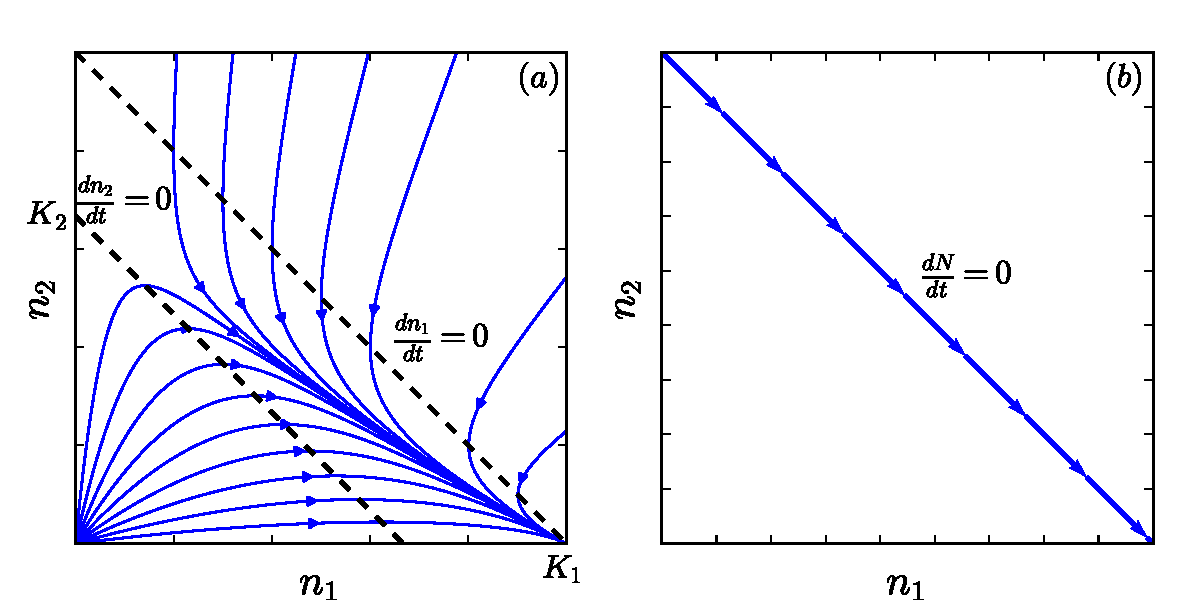
\includegraphics[scale=0.8]{Kplot.pdf}
\caption{\label{fig:Ksel} Phase diagram for the densities of two types $n_1$ and $n_2$ undergoing selection. (a) The logistic model $\frac{dn_1}{dt}=r_1(1-\frac{n_1+n_2}{K_1})n_1$ and $\frac{dn_2}{dt}=r_2(1-\frac{n_1+n_2}{K_2})n_1$ with $r_1=r_2$ and $K_1>K_2$. (b) The constant-$N$, relative fitness description of selection.}
\end{figure}

In light of the complications arising from density-dependence, the assignment of density-independent relative fitnesses has been justified as an approximation that holds when selection is weak and $N$ changes slowly (\citealt{kimura1969natural}; \citealt[pp. 277]{ewens_2004}; \citealt[Chap. 4]{charlesworth_1994}). Under these conditions, $s$ is approximately constant in Eq.~\eqref{eq:canonicalcont}, at least for some number of generations. If $s$ depends only on density, not frequency, this approximate constancy can hold over entire selective sweeps \citep{otto_2011}. 

However, the preceding arguments do not imply that the constant relative fitness idealization of population genetics \textit{only} applies when selection is weak and $N$ is stable (or when selection is actually density-independent). The idealization of assigning relative fitness values to genotypes is powerful, and so it is important to understand the specifics of when and how it succeeds or fails when selection is not weak, or $N$ is not stable. For instance, in wild \textit{Drosophila}, strong seasonally-alternating selection happens concurrently with large ``boom-bust'' density cycles \citep{messer_2016,bergland_14}. Are we compelled to switch to a more ecologically-detailed model of selection based on Malthusian parameters or birth/death rates in this important model system? And if we make this switch, how much ecological detail do we need? 

Here we argue that the simplified models of density-regulated growth mentioned above are misleading in their representation of the interplay between selection and density. This ultimately derives from their failure to account for ``reproductive excess'', that is, an excess of juveniles that experience stronger selection than their adult counterparts \citep{turner1968population}. By allowing selection to be concentrated at a juvenile ``bottleneck'', reproductive excess makes it possible for the density of adults to remain constant even under strong selection. Reproductive excess featured prominently in early debates about the regulation of population density (e.g. \citealt{nicholson_1954}), and also has a long history in evolutionary theory, particularly related to Haldane's ``cost of selection'' \citep{haldane_1957,turner1968population}. Additionally, reproductive excess is implicit in foundational evolutionary-genetic models like the Wright-Fisher, where each generation involves the production of an infinite number of zygotes, of which a constant number $N$ are sampled to form the next generation of adults. Likewise in the Moran model, a juvenile is always available to replace a dead adult every iteration no matter how rapidly adults are dying, and as a result $N$ remains constant. 

Nevertheless, studies of density-dependent selection rarely incorporate reproductive excess. This requires that we model a finite, density-dependent excess, which is substantially more complicated than modeling either zero (e.g. logistic) or infinite (e.g. Wright-Fisher) reproductive excess. Nei's ``competitive selection'' model incorporated a finite reproductive excess to help clarify the ``cost of selection'' \citep{nei1971fertility,nagylaki_1992}, but used an unusual representation of competition based on pairwise interactions defined for at most two different genotypes, and was also restricted to equal fertilities for each genotype. 

In models with detailed age structure, it is usually assumed that the density of a ``critical age group'' mediates the population's response to crowding \citep[pp. 54]{charlesworth_1994}. Reproductive excess is a special case corresponding to a critical pre-reproductive age group. A central result of the theory of density-regulated age-structured populations is that selection proceeds in the direction of increasing equilibrium density in the critical age group \citep[pp. 148]{charlesworth_1994}. This is a form of the classical $K$-selection ideas discussed above, but restricted to the critical age group (juveniles, in this case). The interdependence of pre-reproductive selection and reproductive density is thus overlooked as a result of focusing on density in the critical age group. 

We re-evaluate the validity of the constant relative fitness description of selection in a novel model of density-regulated population growth that has a finite reproductive excess. Our model is inspired by the classic discrete-time lottery model, which was developed by ecologists to study competition driven by territorial contests in reef fishes and plants \citep{sale_77,chesson_1981}, and which has some similarities to the Wright-Fisher model \citep{svardal_2015}. Each type is assumed to have three traits: fecundity $b$, mortality $d$, and competitive ability $c$. In each iteration of the classic lottery model, each type produces a large number of juveniles, such that $N$ remains constant (infinite reproductive excess). Competitive ability $c$ affects the probability of winning a territory, and behaves like a pure relative fitness trait. Thus, fitness involves a product of fertility and juvenile viability akin to standard population genetic models of selection (e.g. \citealt[pp. 185]{crow_1970}). We relax the large-juvenile-number assumption of the lottery model to derive a variable-density lottery with a finite, density-dependent reproductive excess. 

The properties of density-dependent selection in our model are strikingly different from the classical literature discussed above. The strong connection between crowding and selection for greater equilibrium density is broken: selection need not affect density at all. And when it does, the density-independent discrete-time selection equation \eqref{eq:canonicaldisc} is almost exact even for strong selection, provided that any changes in density are driven only by selection (as opposed to large deviations from demogaphic equilibrium), and that selection occurs on only one of the traits $b$, $c$, or $d$. On the flip side, the constant relative fitness approximation fails when strong selection acts concurrently on two or more of these traits, or when the population is far from demographic equilibrium.

\section*{Model}\label{sec:model}

\subsection*{Assumptions and definitions} 

We restrict our attention to asexual haploids, since it is then clearer how the properties of selection are tied to the underlying population ecological assumptions. We assume that reproductively mature individuals (``adults'') require their own territory to survive and reproduce. All territories are identical, and the total number of territories is $T$. Time advances in discrete iterations, each representing the time from birth to reproductive maturity. In a given iteration, the number of adults of the $i$'th type will be denoted by $n_i$, the total number of adults by $N=\sum_i n_i$, and the number of unoccupied territories by $U=T-N$. We assume that the $n_i$ are large enough that stochastic fluctuations in the $n_i$ (drift) can be ignored (with $T$ also assumed large to allow for low type densities $n_i/T\ll 1$). 

\begin{figure}
\centering
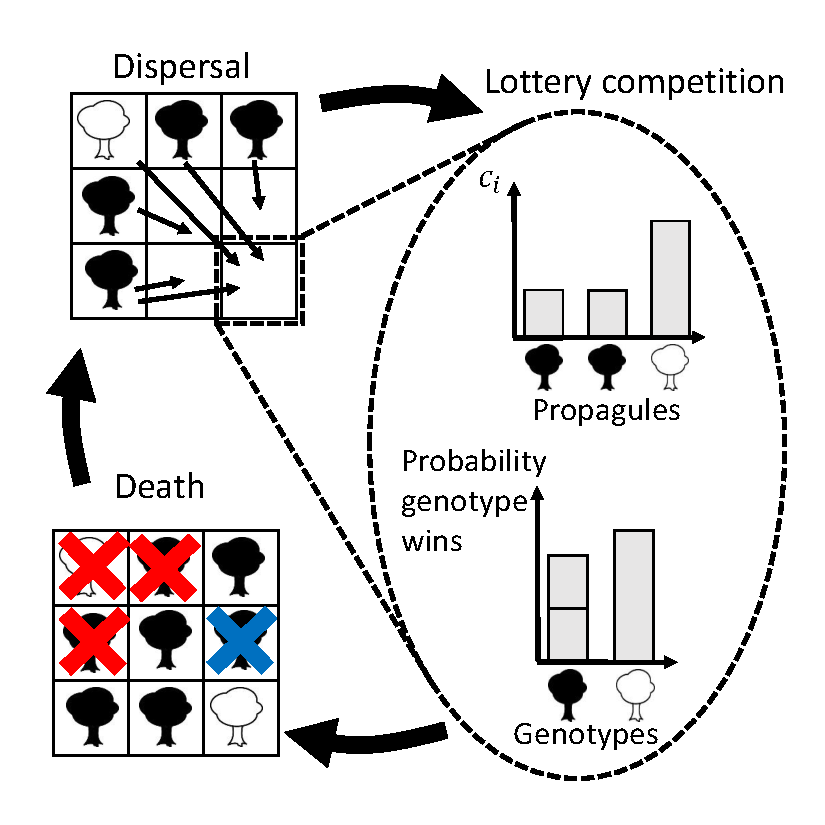
\includegraphics[scale=0.8]{lottery.pdf}
\caption{\label{fig:lottery} One iteration of our model. Propagules are dispersed by adults at random (only those propagules landing on unoccupied territories are shown). Some territories may receive zero propagules. Lottery competition then occurs in each territory that receives more than one propagule (only illustrated in one territory). In a given territory, type $i$ has probability proportional to $c_i x_i$ of winning the territory, where $c_i$ measures competitive ability and $x_i$ is the number of $i$ propagules present. In the illustrated territory, more black propagules are present, but white is a stronger competitor and has a higher probability of winning. Adult deaths make new territories available for the next iteration (red crosses).}
\end{figure}

Each iteration, adults produce propagules which disperse at random, independently of distance from their parents, and independently of each other. We assume that each adult from type $i$ produces $b_i$ propagules on average, so that the mean number of $i$ propagules dispersing to unoccupied territories is $m_i=b_in_iU/T$. The parameter $b_i$ can be thought of as a measure of ``colonization ability'', which combines fertility and dispersal ability \citep{levins_71,tilman_94}. Random dispersal is then modeled using a Poisson distribution $p_i(x_i)=l_i^{x_i} e^{-l_i}/x_i!$ for the number $x_i$ of $i$ propagules dispersing to any particular unoccupied territory, where $l_i=m_i/U$ is the mean propagule density in unoccupied territories. The total propagule density will be denoted $L=\sum_i l_i$.

We assume that adults cannot be ousted by juveniles, so that recruitment to adulthood occurs exclusively in unoccupied territories. When multiple propagules land on the same unoccupied territory, the winner is determined by lottery competition: type $i$ wins a territory with probability $c_i x_i/\sum_i c_i x_i$, where $c_i$ is a constant representing relative competitive ability (Fig. \ref{fig:lottery}). Since the expected fraction of unoccupied territories with propagule composition $x_1,\ldots,x_G$ is $p_1(x_1)\cdots p_G(x_G)$ where $G$ is the number of types present, and type $i$ is expected to win a proportion $c_i x_i/\sum_i c_i x_i$ of these, type $i$'s expected territorial acquisition is given by
\begin{equation}
\Delta_+ n_i=U\sum_{x_1,\ldots,x_G} \frac{c_i x_i}{\sum_i c_i x_i} p_1(x_1)\cdots p_G(x_G). \label{eq:growthsumuncoupled}
\end{equation}
Here the sum only includes territories with at least one propagule present. Since we do not consider random genetic drift here, we will not analyze the fluctuations around these two expectations.

Adult mortality occurs after lottery recruitment at a constant, type-specific per-capita rate $d_i\geq 1$, and can affect adults recruited in the current iteration, such that the new abundance at the end of the iteration is $(n_i+\Delta_+ n_i)/d_i$ (Fig.~\ref{fig:lottery}). In terms of absolute fitness, this can be written as
\begin{equation}
W_i=\frac{1}{d_i}\left(1+\frac{\Delta_+ n_i}{n_i}\right). \label{eq:absfit}
\end{equation}
Here $\frac{\Delta_+ n_i}{n_i}$ is the per-capita rate of territorial acquisition, and $1/d_i$ is the fraction of type $i$ adults surviving to the next iteration.

\subsection*{Connection to the classic lottery model}

In the classic lottery model \citep{chesson_1981}, unoccupied territories are assumed to be saturated with propagules from every type ($l_i\rightarrow \infty$ for all $i$). From the law of large numbers, the composition of propagules in each territory will not deviate appreciably from the mean composition $l_1,l_2,\ldots,l_G$. Type $i$ is thus expected to win a proportion $c_i l_i/\sum_i c_i l_i$ of the $U$ available territories,
\begin{equation}
\Delta_+ n_i=\frac{c_i l_i}{\sum_i c_i l_i}U=\frac{c_i l_i}{\overline{c}L}U, \label{eq:lottery}
\end{equation}
where $\overline{c}=\sum_i c_i m_i/\sum_i m_i$ is the mean competitive ability for a randomly selected propagule. Note that all unoccupied territories are filled in a single iteration of the classic lottery model, whereas our more general model Eq.~\eqref{eq:growthsumuncoupled} allows for territories to be left unoccupied and hence also accommodates low propagule densities.

\section*{Results}

\subsection*{Analytical approximation of the variable-density lottery}

Here we evaluate the expectation in Eq.~\eqref{eq:growthsumuncoupled} to better understand the dynamics of density-dependent lottery competition. Similarly to the classic lottery model, we replace the $x_i$, which take different values in different territories, with ``effective'' mean values. However, since we want to allow for low propagule densities, we cannot simply replace the $x_i$ with the means $l_i$ as in the classic lottery. For a low density type, growth comes almost entirely from territories with $x_i=1$, for which its mean density $l_i\ll 1$ is not representative. We therefore separate Eq.~\eqref{eq:growthsumuncoupled} into $x_i=1$ and $x_i>1$ components, taking care to ensure that the effective mean approximations for these components are consistent with each other (details in Appendix B). The resulting variable-density approximation only requires that there are no large discrepancies in competitive ability (i.e. we do not have $c_i/c_j\gg 1$ for any two types). We obtain
\begin{equation}
\Delta_+ n_i\approx \left[e^{-L}+(R_i+A_i)\frac{c_i}{\overline{c}}\right]l_i U, \label{eq:master}
\end{equation}
where
\begin{equation}
R_i=\frac{\overline{c}e^{-l_i}(1-e^{-(L-l_i)})}{c_i +\frac{\overline{c}L- c_il_i}{L-l_i}\frac{L-1+e^{-L}}{1-(1+L)e^{-L}}},\nonumber \label{eq:Dr}
\end{equation}
and
\begin{equation}
A_i=\frac{\overline{c}(1-e^{-l_i})}{\frac{1-e^{-l_i}}{1-(1+l_i)e^{-l_i}}c_il_i+\frac{\overline{c}L- c_il_i}{L-l_i}\left(L\frac{1-e^{-L}}{1-(1+L)e^{-L}}-l_i\frac{1-e^{-l_i}}{1-(1+l_i)e^{-l_i}}\right)}. \nonumber \label{eq:Da}
\end{equation}

Comparing Eq. \eqref{eq:master} to Eq. \eqref{eq:lottery}, the classic lottery per-propagule success rate $c_i/\overline{c}L$ has been replaced by three separate terms. The first, $e^{-L}$, accounts for propagules which land alone on unoccupied territories; these propagules secure the territories without contest. The second, $R_i c_i/\overline{c}$, represents competitive victories on territories where only a single $i$ propagule lands, together with at least one other propagule from a different type (this term dominates the growth of a rare invader in a high density population and determines invasion fitness). The third term, $A_i c_i/\overline{c}$, represents competitive victories in territories where two or more $i$ type propagules are present. The relative importance of these three terms varies with both the overall propagule density $L$ and the relative propagule frequencies $l_i/L$. If $l_i\gg 1$ for all types, we recover the classic lottery model (only the $A_ic_i/\overline{c}$ term remains, and $A_i\rightarrow 1/L$). 

Fig.~\ref{fig:simcomp} shows that Eq. \eqref{eq:master} and its components closely approximate simulations of our variable-density lottery model over a wide range of propagule densities.  Two types are present, one of which is at low frequency. The growth of the low-frequency type relies crucially on the low-density competition term $R_i c_i/\overline{c}$. On the other hand, $R_i c_i/\overline{c}$ is negligible for the high-frequency type, which depends instead on high density territorial victories. Fig.~\ref{fig:simcomp} also shows the breakdown of the classic lottery model at low propagule densities.

\begin{figure}
\centering
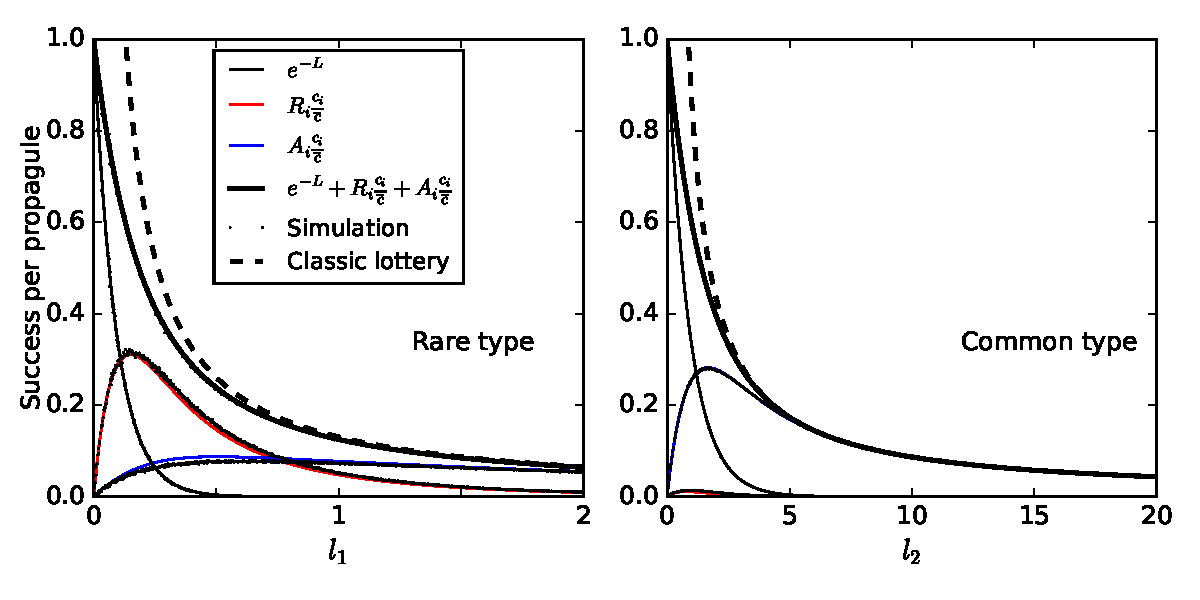
\includegraphics[scale=0.8]{simulationcomparison.pdf}
\caption{\label{fig:simcomp} Comparison of Eq.~\eqref{eq:master}, the classic lottery model, and simulations. The vertical axis is per-propagule success rate for all propagules $\Delta_+ n_i/m_i$, and for the three separate components in Eq.~\eqref{eq:master}. Two types are present with $c_1=1$, $c_2=1.5$ and $l_2/l_1=0.1$. Simulations are conducted as follows: $x_1,x_2$ values are sampled $U=10^5$ times from Poisson distributions with respective means $l_1,l_2$, and the victorious type in each territory is then decided by random sampling weighted by the lottery win probabilities $c_ix_i/(c_1 x_1 + c_2 x_2)$. Dashed lines show the failure of the classic lottery model at low density.} 
\end{figure}

In the special case that all types are competitively equivalent (identical $c_i$), Eq.~\eqref{eq:master} takes a simpler form,
\begin{equation}
\Delta_+ n_i = \frac{l_i}{L}(1-e^{-L})U. \label{eq:masterequalc}
\end{equation}
This formula can also be deduced directly from Eq.~\eqref{eq:growthsumuncoupled}: $1-e^{-L}$ is the fraction of territories that receive at least one propagule under Poisson dispersal, $(1-e^{-L})U$ is the total number of such territories, and type $i$ is expected to receive a fraction $l_i/L$ of these. Total population density thus grows according to
\begin{equation}
\Delta N=(1-e^{-L})U-\sum_i d_i n_i \label{eq:Nmaster}
\end{equation}

\subsection*{Density-dependent selection in the variable-density lottery}

We now outline the basic properties of selection on $b$, $c$ and $d$. The birth and mortality rates $b$ and $d$ are the traits which regulate density; $b$ controls the fraction of unoccupied territories that are contested, while $d$ controls adult mortality. Competitive ability $c$ does not regulate density since it only affects the relative likelihood for each type to win a contested territory. Thus, selection between types which only differ in $c$ occurs without causing $N$ to change (Eq.~\eqref{eq:Nmaster} shows this formally). 

Selection in our variable density lottery model is density-dependent. This means that when two types are present, the discrete-time selection factor $(W_i-W_j)/\overline{W}$ in Eq.~\eqref{eq:canonicaldisc} may depend on $N$. Note that density-dependent selection is sometimes taken to mean a qualitative change in which types are fitter than others at different densities \citep{travis_2013}. While reversal in the order of fitnesses and co-existence driven by density-regulation are possible in our variable-density lottery (a special case of the competition-colonization trade-off; \citealt{levins_71,tilman_94,bolker_99}), questions related to co-existence are tangential to our aims and will not be pursued further here. 

Selection on $c$ is density-dependent, with the strength of selection  peaking at an intermediate density (Fig.~\ref{fig:DDS_lottery}). This intermediate peak occurs because most territories are claimed without contest at low density, whereas at high density few unoccupied territories are available to be contested. 

To see how selection on $b$ and $d$ depend on density, we write Eq.~\eqref{eq:masterequalc} in the alternative form
\begin{equation}
\frac{\Delta_+ n_i}{n_i} = \frac{b_i}{\overline{b}}\frac{1-e^{-\overline{b}N/T}}{N}(T-N), \label{eq:bdensitydependence}
\end{equation}
where we have used that fact that $L=\overline{b}N/T$, and $\overline{b}$ is the population mean $b$. It is then clear that $d$-selection is independent of density, because the density-dependent factor $1 + \frac{\Delta_+ n_i}{n_i}$ in Eq.~\eqref{eq:absfit} is the same for types that differ in $d$ only. On the other hand, the strength of $b$-selection declines with density because the advantage of having greater $b$ gets smaller the fewer territories there are to be claimed (Fig.~\ref{fig:DDS_lottery}). 

\begin{figure}
\centering
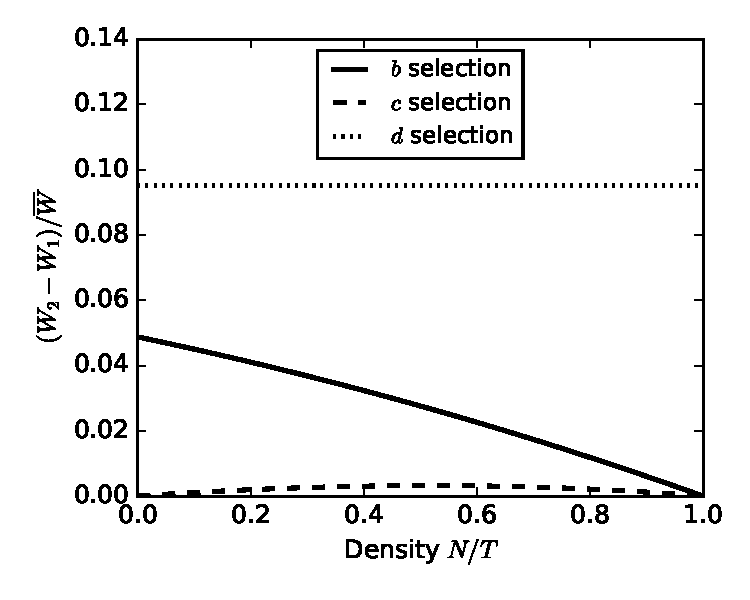
\includegraphics[scale=0.8]{DDS_lottery.pdf}
\caption{\label{fig:DDS_lottery} The density-dependence of selection in our variable-density lottery between an adaptive variant $2$ and a wildtype $1$ with equal frequencies. Here $b_1=1$, $d_1=2$ and $c_1=1$. For $b$-selection we set $b_2=b_1(1+\epsilon)$, and similarly for $c$ and $d$, with $\epsilon=0.1$. $d$-selection is density-independent, $b$-selection gets weaker with lower territorial availability, while $c$-selection initially increases with density as territorial contests become more important, but eventually also declines as available territories become scarce.}
\end{figure}

\subsection*{The response of density to selection; $c$-selection versus $K$-selection}

In this section we discuss the response of density to selection, comparing our variable-density lottery to previous studies of density-regulated populations. Our focus will be on the competitive ability trait $c$, because, as mentioned in the previous section, $c$-selection has no effect on population density even though it affects fitness under crowded conditions. Since this behavior is quite different from selection on more commonly used crowding-sensitivity parameters like $K$ in the logistic model, we start by revisiting MacArthur's $K$-selection argument \citep{macarthur_1967}.

MacArthur considered a population with two types that have densities $n_1$ and $n_2$ subject to density-dependent growth,
\begin{equation}
\frac{d n_1}{d t}=f_1(n_1,n_2)\qquad\frac{d n_2}{d t}=f_2(n_1,n_2). \label{eq:macgeneral}
\end{equation}
The environment is assumed to remain constant apart from changing type densities. The functions $f_1$ and $f_2$ must decline to zero if $n_1$ or $n_2$ are sufficiently large, because the resources required for growth are limited. This defines nullclines $f_1(n_1,n_2)=0$ and $f_2(n_1,n_2)=0$ in $(n_1,n_2)$ space. The outcome of selection is then determined by the relationship between these nullclines. Specifically, a type will be excluded if its nullcline is completely contained in the region bounded by the other type's nullcline. Thus, for a type to have the possibility of persisting, it must be able to keep growing to higher densities than the other type can tolerate in some region of $(n_1,n_2)$ space (Fig.~\ref{fig:Ksel}a).

MacArthur used ``$K$'' to label the four intersection points of the nullclines with the axes, specifically $f_1(K_{11},0)=0$, $f_1(0,K_{12})=0$, $f_2(K_{21},0)=0$ and $f_2(0,K_{22})=0$. These $K$ values determine whether a region of higher-density growth exists for each type, provided that the nullclines are close to being straight lines. Note that only $K_{11}$ and $K_{22}$ are equilibrium densities akin to the $K$ parameter in the logistic model (Fig.~\ref{fig:Ksel}a). The other intersection points, $K_{12}$ and $K_{21}$, are related to competition between types. To be more concrete, in the Lotka-Volterra competition model we have
\begin{align}
f_1(n_1,n_2) = r_1(1-\alpha_{11}n_1-\alpha_{12}n_2)n_1\nonumber\\
f_2(n_1,n_2) = r_2(1-\alpha_{22}n_1-\alpha_{21}n_2)n_2\label{eq:LV}
\end{align}
where $\alpha_{11}=1/K_{11}$ and $\alpha_{22}=1/K_{22}$ measure competitive effects within types, while $\alpha_{12}=1/K_{12}$ and $\alpha_{21}=1/K_{21}$ measure competitive effects between types. Hence, ``fitness is $K$'' in crowded populations \citep[pp. 149]{macarthur_1967} in the sense that selection either favors the ability to keep growing at ever higher densities (moving a type's own nullcline outwards), or the ability to suppress the growth of competitors at lower densities (moving the nullcline of competitors inwards). This general idea is much broader than selection for greater equilibrium density \citep{gill_1974}.

\begin{figure}
\centering
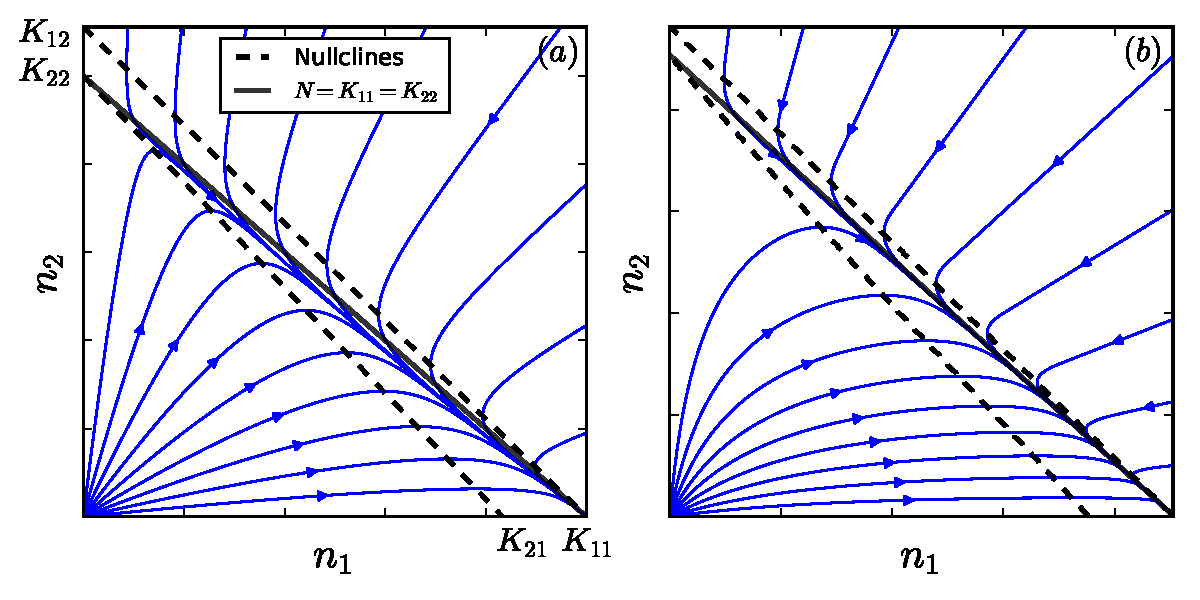
\includegraphics[scale=0.8]{LVvslottery.pdf}
\caption{\label{fig:LVvslottery} Selection between types with identical equilibrium density but different inter-type competitive ability. (a) Lotka-Volterra competition (Eq.~\ref{eq:LV}) with $r_1=r_2=1$, $\alpha_{11}=\alpha_{22}=1$, $\alpha_{12}=0.9$ and $\alpha_{21}=1.2$. Trajectories do not follow the line $N=K_{11}=K_{22}$. (b) Lottery competition (Eq.~\ref{eq:master}) with $b_1=b_2=5$, $d_1=d_2=1.1$ and $c_1/c_2=5$. Trajectories converge on the line $N=K_{11}=K_{22}$.}
\end{figure}

Compared to simple birth-death models \citep{kostitzin_1939} or variants of the logistic \citep{roughgarden_1979}, the Lotka-Volterra model clearly distinguishes between intra- and inter-type competitive effects. Thus, when selection acts on inter-type competitive effects, one type can displace another without having a greater equilibrium density (Fig.~\ref{fig:LVvslottery}a). This has been termed ``$\alpha$-selection'' to distinguish it from $K$-selection, which involves intra-type competitive effects and changes in equilibrium density \cite{gill_1974,joshi_2001}. Although the initial and final densities of an $\alpha$-selection sweep are the same, density nevertheless does change transiently in the Lotka-Volterra model (constant density only occurs for a highly restricted subset of $r$ and $\alpha$ values; further details in Appendix C; also see \citealt{mallet_2012,smouse_1976}). Intuitively, for one type to exclude the other, competitive suppression of growth between types must be stronger than competitive suppression of growth within types, causing $N$ to dip over a sweep (Fig.~\ref{fig:LVvslottery}a). 

By contrast, density trajectories for $c$-selection in our variable-density lottery converge on a line of constant equilibrium density (Fig.~\ref{fig:LVvslottery}b). This means that once the population reaches demographic equilibrium, it behaves indistinguishably from a constant-$N$ relative fitness model (Fig.~\ref{fig:Ksel}b). This complete uncoupling of density from $c$-selection arises due to the presence of an excess of propagules which pay the cost of selection without affecting adult density \citep{nei1971fertility}. As a result, the density-independent Eq.~\eqref{eq:canonicaldisc} holds in demographic equilibrium even though $c$-selection is density-dependent.

\subsection*{Density-regulating traits and the threat of strong selection}

For Eq.~\eqref{eq:canonicaldisc} to break down, the selection factor $(W_i-W_j)/\overline{W}$ must depend on density. As shown in Fig.~\ref{fig:DDS_lottery}, this is not the case for $d$. Eq.~\eqref{eq:canonicaldisc} also holds when the population is at demographic equilibrium and density is unaffected by the outcome of selection; as discussed in the previous section, the latter is the case for $c$-selection in our model. Thus, to threaten Eq.~\eqref{eq:canonicaldisc}, we require selection to be density-dependent, and also density to be changing. This can obviously occur if density-dependent selection is occurring in a population far from demographic equilibrium. In this case the validity of Eq.~\eqref{eq:canonicaldisc} depends on the specifics of the rate and magnitude of demographic change (we return to this in the Discussion). However, Eq.~\eqref{eq:canonicaldisc} can be threatened even in demographically-stable populations if a density-regulating trait is subject to density-dependent selection, as is the case for $b$ in our variable-density lottery. 

Before we discuss the $b$ trait, it is helpful to summarize how Eq.~\eqref{eq:canonicalcont} breaks down in a simpler continuous-time birth-death model \citep{kostitzin_1939} 
\begin{equation}
\frac{d n_i}{dt}=(b_i -\delta_iN) n_i. \label{eq:simplebirthdeath}
\end{equation}
Here $\delta_i$ is per-capita mortality due to crowding (for simplicity, there are no deaths when uncrowded). Starting from a type $1$ population in equilibrium, a variant with $\delta_2=\delta_1(1-\epsilon)$ has density-dependent selection coefficient $s=\epsilon \delta_1 N$ in Eq.~\eqref{eq:canonicalcont}, which will change over the course of the sweep as $N$ shifts from its initial type $1$ equilibrium to a type $2$ equilibrium. From Eq.~\eqref{eq:simplebirthdeath}, the equilibrium densities at the beginning and end of the sweep are $N_{\rm initial}=b_1/\delta_1$ and $N_{\rm final}=b_1/(\delta_1(1-\epsilon))=N_{\rm initial}/(1-\epsilon)$ respectively, and so $s_{\rm initial}= \epsilon b_1$ and $s_{\rm final}=s_{\rm initial}/(1-\epsilon)$. Consequently, substantial deviations from Eq.~\eqref{eq:canonicalcont} occur if there is sufficiently strong selection on $\delta$ (Fig.~\ref{fig:strengthofselection}; \citealt{kimura1969natural,crow_1970}).

\begin{figure}
\centering
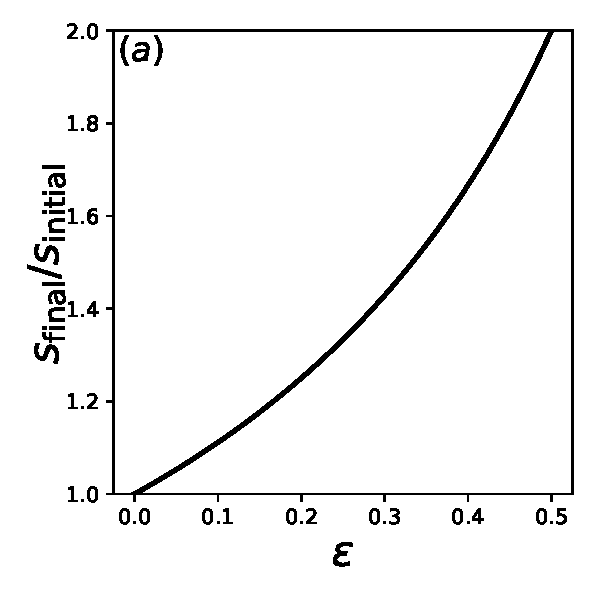
\includegraphics[scale=0.8]{strengthofselection.pdf}
\caption{\label{fig:strengthofselection} (a) Change in the selection coefficient between the beginning and end of a sweep of a type that experiences proportionally $1-\epsilon$ fold fewer crowding-induced deaths. The population is in demographic equilibrium at the start and end of the sweep. (b) Example equilibrium-to-equilibrium sweep.}
\end{figure}

Equilibrium-to-equilibrium $b$-sweeps in our variable-density lottery are qualitatively different from $\delta$ sweeps in this simpler birth-death model, because greater $b$ not only means more propagules contesting territories, but also more territories being contested. Together, the net density-dependent effect on $b$-selection is negligible: in a single-type equilibrium we have $W_i=1$ and $b_i/\overline{b}=1$, and hence the density-dependence factor $f(\overline{b},N)=\frac{1-e^{-\overline{b}N/T}}{N}(T-N)$ in Eq.~\eqref{eq:bdensitydependence} has the same value $d_i-1$ at the beginning and end of a $b$-sweep. During the sweep there is some deviation in $f(\overline{b},N)$, but this deviation is an order of magnitude smaller than for a $\delta$ sweep (the density-dependent deviation in Fig.~\ref{fig:strengthofselection} is of order $\epsilon$, whereas the analogous effect for $b$ sweep in our variable-density lottery is only of order $\epsilon^2$; see Appendix D for details). Since selection must already be strong for a $\delta$-sweep to threaten Eq.~\eqref{eq:canonicalcont}, the density-independent model applies effectively exactly for equilibrium $b$-sweeps.

If selection acts simultaneously on more than one trait in our variable-density lottery, then evolution in a density-regulating trait can drive changes in the strength of selection on a trait subject to density-dependent selection (Fig.~\ref{fig:multiple}). This can produce behavior analogous to selection on $\delta$ in Fig.~\ref{fig:strengthofselection}. 

\begin{figure}
\centering
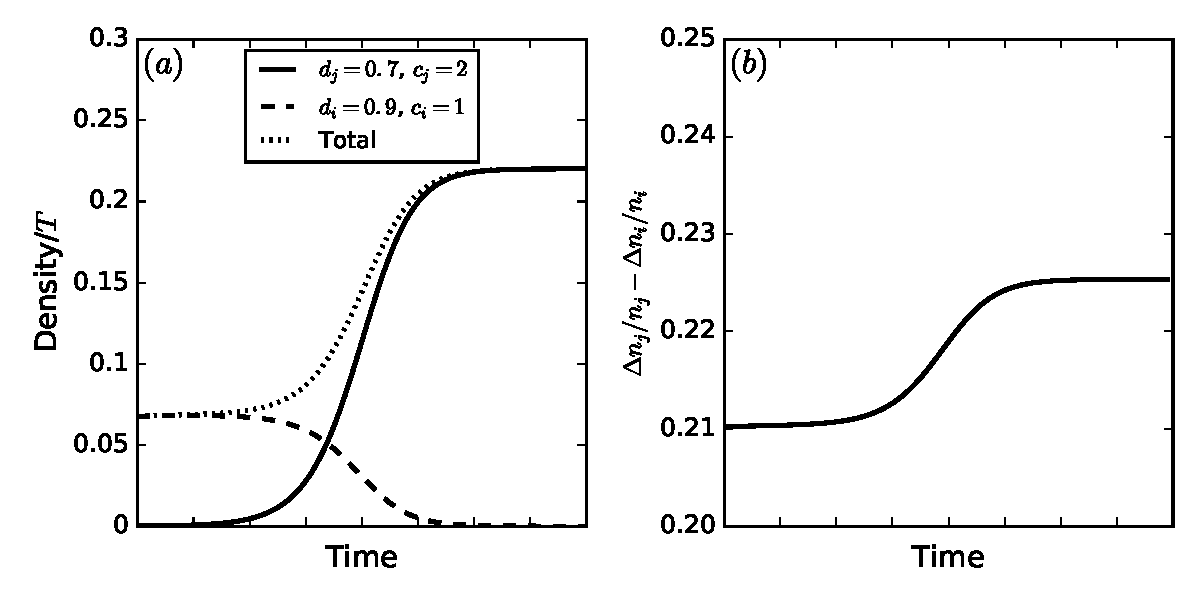
\includegraphics[scale=0.8]{multiple.pdf}
\caption{\label{fig:multiple} Simultaneous selection on $d$ and $c$ in our variable-density lottery model as predicted by Eq.~\eqref{eq:master}. Selection is not constant over the sweep because $d$ is density-regulating and $c$ is density-dependent.}
\end{figure}

\section*{Discussion}

Summarizing the properties of selection in our variable-density lottery model: (i) $c$-selection is density-dependent, but $c$ does not regulate density; (ii) $d$ regulates density, but $d$-selection is density-independent; (iii) $b$ regulates density and $b$-selection is density-dependent. Yet, despite the differences between $b$, $c$ and $d$, in a constant environment selection that only involves one of these traits obeys the density-independent relative fitness description of selection almost exactly. When strong selection acts on more than one of $b$, $c$ and $d$ (Fig.~\ref{fig:multiple}), the constant-$s$ approximation breaks down. The $c$ and $d$ traits exemplify the two distinct directions in which density and selection can interact: selection may depend on density, and density may change in response to ongoing selection \citep{prout_1980}. The combination of both is necessary to threaten the constant-$s$ approximation. Remarkably, the $b$ trait demonstrates that the combination is not sufficient; the density-dependence of $b$-selection effectively disappears over equilibrium-to-equilibrium $b$-sweeps. 

Selection in the variable-density lottery is quite different from classical density-dependent selection (see ``Introduction'' and ``The response of density to selection; $c$-selection versus $K$-selection''). In the latter, only one life-history stage is represented, and the effects of crowding appear as a reduction in absolute fitness that only depends on the type densities at this life-history stage (e.g. the $n_i^2$ and $n_in_j$ terms in the Lotka-Volterra equation). Selection in crowded populations takes broadly one of two forms: selection for greater carrying capacity ($K$-selection) or selection on competition coefficients ($\alpha$-selection). These are both ``$\delta$-like''  in the sense that selection depends on density and also causes density to change ($\delta$ is defined in Eq.~\eqref{eq:simplebirthdeath}). Strong selection is therefore sufficient for Eq.~\eqref{eq:canonical} to break down (Fig.~\ref{fig:strengthofselection}), and no distinction is made between density-regulating and density-dependent traits.

The distinctive properties of selection in the variable-density lottery arise from a reproductive excess which appears when the number of propagules is greater than the number of available territories. Then only $\approx 1/L$ of the juveniles contesting unoccupied territories survive to adulthood. Unlike the role of adult density $n_i$ in single-life-stage models, it is the propagule densities $l_i$ that represent the crowding that drives competition. Reproductive excess produces relative contests in which fitter types grow at the expense of others by preferentially filling the available adult ``slots''. The number of available slots can remain fixed or change independently of selection at the juvenile stage. By ignoring reproductive excess, single life-stage models are biased to have total population density be more sensitive to ongoing selection. In this respect, the viability selection heuristics that are common in population genetics \cite[pp. 61]{gillespie_2004} actually capture an important ecological process without making the full leap to complex age-structured models.

Looking beyond the variable-density lottery, it is not clear which forms of crowding-induced selection are more likely to occur in nature. Even if reproductive excesses are ubquitous, strictly relative $c$-like traits could pleiotropically interact with density-regulating traits so often that $\delta$-like behavior is prevalent. For instance, in the case in the case of well-mixed indirect exploitation competition for consumable resources, the $R^*$ rule suggests that competitive ability is intimately linked to equilibrium resource density, and hence that $\delta$-like behavior would be prevalent. However, this conclusion is sensititive to the assumptions of well-mixed resource competition models. Spatial localization of consumable resources (e.g. for plants due to restricted movement of nutrients through soils) will tend to create territorial contests similar to the lottery model, where resource competition only occurs locally and can be sensitive to contingencies such as the timing of propagule arrival \cite{bolker_99}. In this case, resource competition is effectively subsumed into a territorial competitive ability trait akin to $c$, which would likely affect $N$ much more weakly than suggested by the $R^*$ rule (assuming no pleiotropic interactions with $b$ or $d$). 

Moreover, even in well mixed populations, competition does not only involve indirect exploitation of shared resources, but also direct interference. Interference competition can dramatically alter the dynamics of resource exploitation \cite{case_1974,amarasekare_2002}, and is more likely than the exploitation of shared resource pools to involve relative contests akin to $c$-selection. For instance, sexual selection can be viewed as a form of relative interference competition between genotypes. Thus, \textit{a priori} we should not expect crowding in nature to only involve selection that is $\delta$-like. Other forms of selection like $c$-selection (that is, strictly relative traits in density-regulated populations) are also likely to be important. Note that in the classical density-dependent selection literature, interference competition is closely associated with $\alpha$-selection and the idea that selection need not affect equilibrium density \cite{gill_1974}. However, as explained above, $\alpha$-selection does transiently affect population density and can therefore be regarded as $\delta$-like.

The above findings underscore that the most serious threat to the constant-$s$ approximation arises due to deviations from demographic equilibrium as a result of changes in the demographic rates of the types already present i.e. as a result of a temporally-variable environment. While transient deviations from demographic equilibrium driven by the appearance of new types can also threaten the constant-$s$ approximation, they require strong selection that is both density-dependent and affects a density-regulating trait (and even then the constant-$s$ approximation may hold). In contrast, temporally-variable environments can dramatically alter frequency trajectories for individual sweeps (e.g. Fig. 9.5 in \cite{otto_2011}; Fig. 5 in \cite{mallet_2012}), as well as the long-term outcomes of selection \citep{lande_2009}. 

This suggests that in systems like the wild \textit{Drosophila} example mentioned in the Introduction, there is indeed no choice but to abandon relative fitness. Our variable-density lottery could provide a useful starting point for analyzing evolution in this and other far-from-equilibrium situations for two reasons: 1) the $b$, $c$, $d$ trait scheme neatly distinguishes between different aspects of the interplay between density and selection; 2) lottery models in general are mathematically similar to the Wright-Fisher model, which should facilitate the analysis of genetic drift when $N$ is unstable.

\bibliographystyle{abbrvnat}
\bibliography{reference} 

\section*{Appendix A: Growth equation derivation}

In this appendix we derive Eq.~\eqref{eq:master}. Following the notation in the main text, the Poisson distributions for the $x_i$ (or some subset of the $x_i$) will be denoted $p$, and we use $P$ as a general shorthand for the probability of particular outcomes.

We start by separating the right hand side of Eq.~\eqref{eq:growthsumuncoupled} into three components
\begin{equation}
\Delta_+ n_i = \Delta_u n_i+\Delta_r n_i+\Delta_a n_i,\label{eq:delt_decomp}
\end{equation}
which vary in relative magnitude depending on the propagule densities $l_i$. The first component, $\Delta_u n_i$, accounts for territories where only one focal propagule is present ($x_i=1$ and $x_j=0$ for $j\neq i$; $u$ stands for ``uncontested''). The proportion of territories where this occurs is $l_i e^{-L}$, and so 
\begin{equation}
\Delta_u n_i=Ul_i e^{-L}=m_i e^{-L}.
\end{equation}

The second component, $\Delta_r n_i$, accounts for territories where a single focal propagule is present along with at least one non-focal propagule ($x_i=1$ and $X_i\geq 1$ where $X_i=\sum_{j\neq i} x_j$ is the number of nonfocal propagules; $r$ stands for ``rare''). The number of territories where this occurs is $Up_i(1)P(X_i\geq 1)=m_i e^{-l_i}(1-e^{-(L-l_i)})$. Thus 
\begin{equation}
\Delta_r n_i = m_i e^{-l_i}(1-e^{-(L-l_i)})\left\langle  \frac{c_i}{c_i +\sum_{j\neq i} c_j x_j } \right\rangle_{\tilde{p}},  \label{eq:deltr}
\end{equation}
where $\langle \rangle_{\tilde{p}}$ denotes the expectation with respect to the probability distribution $\tilde{p}$ of nonfocal propagule abundances $x_j$, in those territories where exactly one focal propagule, and at least one non-focal propagule, landed. 

The final contribution, $\Delta_a n_i$, accounts for territories where two or more focal propagules are present ($x_i\geq 2$; $a$ stands for ``abundant"). Similar to Eq.~\eqref{eq:deltr}, we have 
\begin{equation}
\Delta_a n_i=U(1-(1+l_i)e^{-l_i})\left\langle \frac{c_i x_i}{\sum_j c_j x_j} \right\rangle_{\hat{p}}\label{eq:delta}
\end{equation}
where $\hat{p}$ is the probability distribution of both focal and nonfocal propagule abundances in those territories where at least two focal propagules landed. 

To derive Eq.~\eqref{eq:master} we approximate the expectations in Eq.~\eqref{eq:deltr} and Eq.~\eqref{eq:delta} by replacing $x_i$ and the $x_j$ with ``effective'' mean values as follows 
\begin{equation}
\left\langle\frac{c_i}{c_i +\sum_{j\neq i} c_j x_j}\right\rangle_{\tilde{p}}\approx \frac{c_i}{c_i +\sum_{j\neq i} c_j \langle x_j\rangle_{\tilde{q}}}.\label{eq:meanfieldr}
\end{equation}
\begin{equation}
\left\langle \frac{c_i x_i}{\sum_j c_j x_j} \right\rangle_{\hat{p}}\approx  \frac{c_i \langle x_i \rangle_{\hat{q}}}{\sum_j c_j \langle x_j\rangle_{\hat{q}}}.\label{eq:meanfielda}
\end{equation}
Here the effective means $\langle \rangle_{\tilde{q}}$ and $\langle \rangle_{\hat{q}}$ are taken with respect to new distributions $\tilde{q}$ and $\hat{q}$, respectively. In the following subsection we define $\tilde{q}$ and $\hat{q}$ and explain our reasoning for using these distributions to take the effective means. 

\subsection*{The effective distributions $\tilde{q}$ and $\hat{q}$}

The approximations \eqref{eq:meanfieldr} and \eqref{eq:meanfielda} must be consistent between rare and common types. To illustrate, suppose that two identical types (same $b$, $c$ and $d$) are present, with low $l_1\ll 1$ and high density $l_2\approx L\gg 1$ respectively. Since $L$ is large, uncontested territories make up a negligible fraction of the total. The rare type grows almost entirely due to $\Delta_r n_1$, while the common type grows almost entirely due to $\Delta_a n_2$. To ensure consistency, the approximate per-capita growth rates implied by the approximations \eqref{eq:meanfieldr} and \eqref{eq:meanfielda} must be equal $\Delta_r n_1/m_1 = \Delta_a n_2/m_2$. Even small violations of this consistency condition would mean exponential growth of one type relative to the other. This behavior is clearly pathological, because any single-type population can be arbitrarily partitioned into identical rare and common subtypes. Thus,   predicted growth or decline would depend on an arbitrary assignment of rarity.

For example, suppose that we use $\tilde{p}$ and $\hat{p}$ to calculate the effective means. The right hand side of Eq. \eqref{eq:meanfieldr} is then approximately $1/(L+1)$, and since $l_1\ll 1$ and $L\gg 1$ we have $\Delta_r n_1 \approx 1/(L+1)$ in Eq.~\eqref{eq:deltr}. Similarly, for the common type, $\sum_j \langle x_j\rangle_{\hat{p}} = L$ in Eq. \eqref{eq:meanfielda}, and so $\Delta_a n_2 \approx 1/L$. Thus, the identical rare type is  pathologically predicted to decline in frequency.

The effective distributions $\tilde{q}$ and $\hat{q}$ are devised to avoid this pathology. The idea is to make the approximation that the distribution for the total number of propagules per territory is the same in all territories. This is only an approximation because conditioning on focal propagules being present does change the distribution of $X$ in the corresponding subset of territories (in the above example, the mean propagule density across all territories is $L$, but in the territories responsible for the growth of the rare type we have $\langle X \rangle_{\tilde{p}}=L+1$). 

More formally, let ${\mathbf x}$ denote the vector of propagule abundances $(x_1,\ldots,x_G)$ in a given territory, and ${\mathbf x_i}=(x_1,\ldots,x_{i-1},x_{i+1}\ldots,x_G)$ similarly denote the vector of non-focal abundances, so that $p({\mathbf x_i})=p_1(x_1)\cdots p_{i-1}(x_{i-1})p_{i+1}(x_{i+1})\cdots p_G(x_G)$. The corresponding total propagule numbers are denoted $X=\sum_j x_j$ and $X_i=X-x_i$. Then, in territories where one focal propagule and at least one non-focal propagule are present, the effective distribution is defined by 
\begin{equation}
\tilde{q}({\mathbf x_i})=\sum_{X=2}^{\infty}P(X|X\geq 2) p({\mathbf x_i}|X_i=X-1),
\end{equation}
where the total number of propagules $X$ follows a Poisson distribution with mean $L$, and $P(X|X\geq 2)=P(X)/P(X\geq 2)=P(X)/(1-(1+L)e^{-L})$. Similarly, in territories where more than one focal propagule is present, the effective distribution is defined by 
\begin{equation}
\hat{q}({\mathbf x})=\sum_{X=2}^{\infty}P(X|X\geq 2) p({\mathbf x}|x_i\geq 2, X).
\end{equation}
 
\subsection*{Calculating the effective means}

Here we calculate the effective means, starting with the $\Delta_r n_i$ component. We have
\begin{align}
\langle x_j \rangle_{\tilde{q}}&=\sum_{\mathbf x_i} \tilde{q}({\mathbf x_i})x_j\nonumber\\
&=\frac{1}{1-(1+L)e^{-L}}\sum_{X=2}^{\infty} P(X) \sum_{\mathbf x_i} p({\mathbf x_i}|X_i=X-1)x_j.
\label{eq:raremonster1}
\end{align}
The inner sum over ${\mathbf x_i}$ is the mean number of propagules of a given nonfocal type $j$ that will be found in a territory which received $X-1$ nonfocal propagules in total, which is equal to $\frac{l_j}{L-l_i}(X-1)$. Thus, 
\begin{align}
\langle x_j \rangle_{\tilde{q}}&=\frac{l_j}{1-(1+L)e^{-L}}\frac{1}{L-l_i}\sum_{X=2}^{\infty} P(X) (X-1)\nonumber\\
&=\frac{l_j}{1-(1+L)e^{-L}}\frac{L-1+e^{-L}}{L-l_i},
\label{eq:meanxjrare}
\end{align}
where the last line follows from $\sum_{X=2}^{\infty} P(X)(X-1)=\sum_{X=1}^{\infty} P(X)(X-1)=\sum_{X=1}^{\infty} P(X)X-\sum_{X=1}^{\infty}P(X)$. Substituting Eqs.~\eqref{eq:meanfieldr} and \eqref{eq:meanxjrare} into Eq.~\eqref{eq:deltr}, we obtain
\begin{equation}
\Delta_r n_i\approx m_i R_i\frac{c_i}{\overline{c}}, \label{eq:deltrfinal}
\end{equation}
where $R_i$ is defined in Eq.~\eqref{eq:Dr}.

Turning now to the $\Delta_a n_i$ component, the mean focal abundance is 
\begin{align}
\langle x_i \rangle_{\hat{q}}&=\sum_{\mathbf x} \hat{q}({\mathbf x}) x_i\nonumber \\
&=\sum_{x_i} p(x_i|x_i\geq 2)x_i \nonumber\\
&=\frac{1}{1-(1+l_i)e^{-l_i}}\sum_{x_i\geq 2} p(x_i)x_i\nonumber\\
&=l_i\frac{1-e^{-l_i}}{1-(1+l_i)e^{-l_i}}.
\end{align}
For nonfocal types $j\neq i$, we have
\begin{align}
\langle x_j \rangle_{\hat{q}}&=\sum_{X=2}^{\infty}P(X|X\geq 2)\sum_{\mathbf x}  p({\mathbf x}|x_i\geq 2,X) x_j\nonumber\\
&=\sum_{X=2}^{\infty}P(X|X\geq 2)\sum_{x_i} p(x_i|x_i\geq 2,X) \sum_{\mathbf x_i}  p(\mathbf x_i|X_i=X-x_i) x_j\nonumber\\
&=\sum_{X=2}^{\infty}P(X|X\geq 2)\sum_{x_i}p(x_i|x_i\geq 2,X) \frac{l_j(X-x_i)}{L-l_i} \nonumber\\
&=\frac{l_j}{L-l_i}\left[\sum_{X=2}^{\infty}P(X|X\geq 2)X - \sum_{x_i}p(x_i|x_i\geq 2) x_i \right]\nonumber\\
&=\frac{l_j}{L-l_i}\left( L\frac{1-e^{-L}}{1-(1+L)e^{-L}}- l_i\frac{1-e^{-l_i}}{1-(1+l_i)e^{-l_i}}\right).
\end{align}
In going from line 2 to 3, we used the same logic used to evaluate the inner sum in Eq.~\eqref{eq:raremonster1}, and in going from 3 to 4 we have separately evaluated the contributions from the $X$ and $x_i$ terms in the numerator. Combining these results with Eqs.~\eqref{eq:delta} and \eqref{eq:meanfielda}, we obtain
\begin{equation}
\Delta_a n_i=m_i A_i \frac{c_i}{\overline{c}},
\end{equation}
where $A_i$ is defined in Eq.~\eqref{eq:Da}.

\subsection*{Approximation limits}

Eq.~\eqref{eq:meanfieldr} and \eqref{eq:meanfielda} must not only be consistent with each other, they must also be individually good approximations. Here we evaluate these approximations.

The fundamental requirement for making the replacement in Eqs.~\eqref{eq:meanfieldr} and \eqref{eq:meanfielda} is that we can ignore the fluctuations in the $x_i$ and hence replace them with a constant effective mean value. Mathematically, we require that the standard deviations $\sigma_{\tilde{q}}(\sum_{j\neq i} c_j x_j)$ and $\sigma_{\hat{q}}(\sum_j c_j x_j)$ must be sufficiently small compared to the corresponding means $\langle\sum_{j\neq i} c_j x_j\rangle_{\tilde{q}}$ and $\langle\sum_j c_j x_j\rangle_{\hat{q}}$ in Eqs.~\eqref{eq:meanfieldr} and \eqref{eq:meanfielda} respectively.  

To evaluate these standard deviations, we will work with $\tilde{p}$ and $\hat{p}$ distributions instead of $\tilde{q}$ and $\hat{q}$. This is mathematically much simpler because the $x_i$ are independent under $\tilde{p}$ and $\hat{p}$, and is justified by the fact that $\tilde{p}$ and $\hat{p}$ are closely related to $\tilde{q}$ and $\hat{q}$ respectively, and so we expect the relevant means and standard deviations will be similar.

Starting with Eq.~\eqref{eq:meanfieldr}, we have $\langle x_j \rangle_{\tilde{p}}=l_j/C$, where $C=1-e^{-(L-l_i)}$, and the corresponding variances and covariances are given by
\begin{align}
\sigma_{\tilde{p}}^2(x_j)&=\langle x_j^2 \rangle_{\tilde{p}}-\langle x_j \rangle_{\tilde{p}}^2\nonumber\\
&=\frac{l_j^2 + l_j}{C}-\frac{l_j^2}{C^2}\nonumber \\
&=\left(1-\frac{1}{C}\right)\frac{l_j^2}{C}+\frac{l_j}{C},\label{eq:varr}
\end{align}
and
\begin{align}
\sigma_{\tilde{p}}(x_j,x_k)&=\langle x_j x_k \rangle_{\tilde{p}}-\langle x_j \rangle_{\tilde{p}}\langle x_k \rangle_{\tilde{p}}\nonumber\\
&=\frac{1}{C}\langle x_j x_k \rangle_p-\frac{l_jl_k}{C^2}\nonumber\\
&=\left(1-\frac{1}{C}\right)\frac{l_j l_k}{C}\qquad\qquad j\neq k. \label{eq:covr}
\end{align} 
Note that $1-1/C$ is negative because $C<1$. Decomposing the variance in $\sum_{j\neq i} c_j x_j$,
\begin{equation}
\sigma_{\tilde{p}}^2(\sum_{j\neq i} c_j x_j)=\sum_{j\neq i}\left[c_j^2\sigma_{\tilde{p}}^2(x_j)+2\sum_{k>j, k\neq i}c_j c_k\sigma_{\tilde{p}}(x_j,x_k)\right],\label{eq:vartotr}
\end{equation}
we obtain 
\begin{equation}
\frac{\sigma(\sum_{j\neq i} c_j x_j)}{\langle\sum_{j\neq i} c_j x_j\rangle}=C^{1/2}\frac{\left(\sum_{j\neq i}c_j^2 l_j+(1-\frac{1}{C})\left(\sum_{j\neq i}c_j l_j\right)^2 \right)^{1/2}}{\sum_{j\neq i}c_j l_j}. \label{eq:cvr}
\end{equation}

Eq.~\eqref{eq:cvr} reveals two key points. First, when the $c_j$ have similar magnitudes (their ratios are of order one), Eq.~\eqref{eq:meanfieldr} is an excellent approximation. In this case, the right hand side of Eq.~\eqref{eq:cvr} is approximately equal to $C^{1/2}\left(\frac{1}{L-l_i}+1-\frac{1}{C}\right)^{1/2}$, which is small for both low and high nonfocal densities. The worst case scenario occurs when $L-l_i$ is of order one, and it can be directly verified that Eq.~\eqref{eq:meanfieldr} is then still a good approximation (see Fig.~\ref{fig:approx_details}). Second, if some of the $c_j$ are much larger than the others, the relative fluctuations in $\sum_{j\neq i} c_j x_j$ can be large. Specifically, in the presence of a rare,  strong competitor ($c_j l_j\gg c_{j'} l_{j'}$ for all other nonfocal types $j'$, and $l_j\ll 1$), then the right hand side of Eq. \eqref{eq:cvr} can be large and we cannot make the replacement Eq.~\eqref{eq:meanfieldr}. Fig.~\ref{fig:approx_details} shows the breakdown of the effective mean approximation when the are large differences in $c$. 

\begin{figure}
\centering
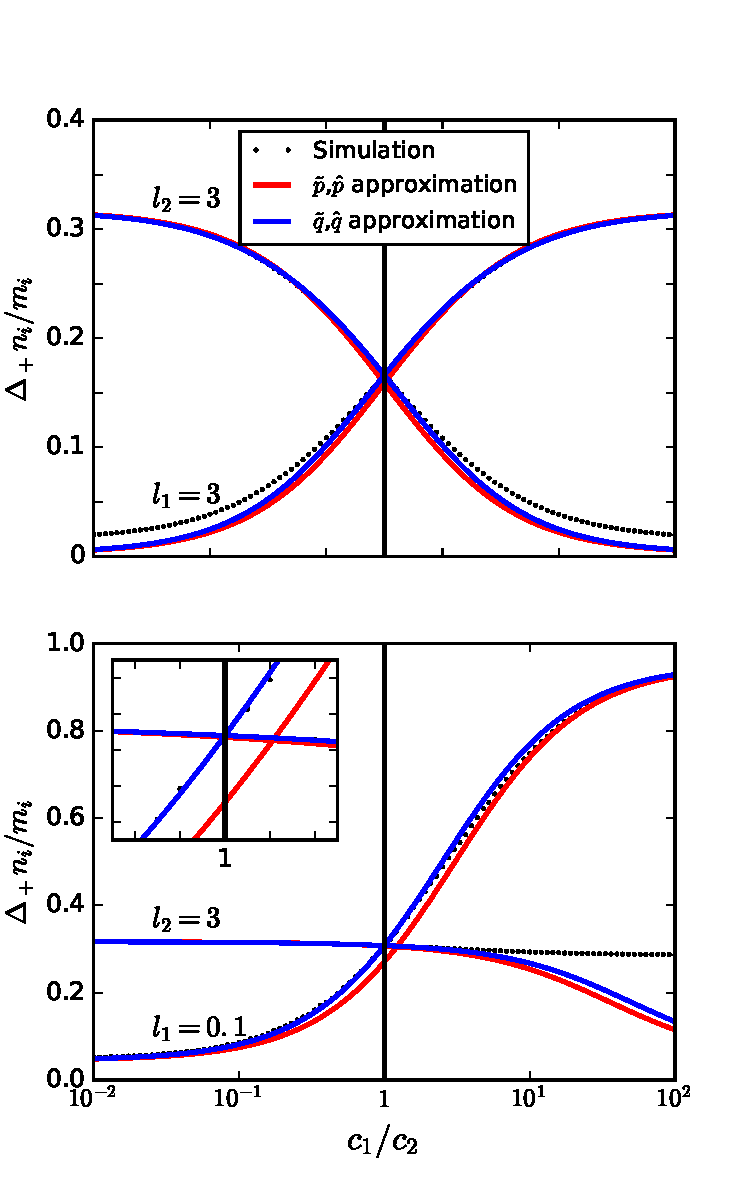
\includegraphics[scale=0.8]{approx_details.pdf}
\caption{\label{fig:approx_details} Comparison of our $\tilde{q}$,$\hat{q}$ approximation with simulations, and also with the naive $\tilde{p}$,$\hat{p}$ approximation, as a function of the relative $c$ difference between two types. Our approximation breaks down in the presence of large $c$ differences. The inset shows the pathology of the $\tilde{p}$,$\hat{p}$ approximation --- growth rates are not equal in the neutral case $c=1$. Simulation procedure is the same as in Fig.~\ref{fig:simcomp}, with $U=10^5$.}
\end{figure}

Turning now to Eq.~\eqref{eq:meanfielda}, all covariances between nonfocal types are now zero, so that $\sigma_{\hat{p}}^2(\sum c_j x_j)=\sum c_j^2 \sigma_{\hat{p}}^2(x_j)$, where $\sigma_{\hat{p}}^2(x_j)=l_j$ for $j\neq i$. Here  
\begin{equation}
\sigma_{\hat{p}}^2(x_i)=\frac{l_i}{D}\left(l_i+1-e^{-l_i}-\frac{l_i}{D}\left(1-e^{-l_i}\right)^2\right),
\end{equation}
where $D= 1-(1+l_i)e^{-l_i}$, and 
\begin{equation}
\frac{\sigma_{\hat{p}}(\sum c_j x_j)}{\langle\sum c_j x_j\rangle} = \frac{\left(\sum_{j\neq i} c_j^2 l_j + c_i^2 \sigma_{\hat{p}}^2(x_i)\right)^{1/2}}{\sum_{j\neq i} c_j l_j + c_i l_i (1-e^{-l_i})/D} \label{eq:cva}.
\end{equation}

Similarly to Eq.~\eqref{eq:cvr}, the right hand side of Eq. \eqref{eq:cva} is small for both low and high nonfocal densities. Again, the worst case scenario occurs when $l_i$ and $L-l_i$ are of order $1$, but Eq.~\eqref{eq:meanfielda} is still a good approximation in this case. Again, the approximation breaks down in the presence of a rare, strong competitor (Fig.~\ref{fig:approx_details}).

\section*{Appendix B: Total density in the Lotka-Volterra competition model}

Here we show that under the Lotka-Volterra model of competition, total density $N$ does not in general remain constant over a selective sweep in a crowded population even if the types have the same equilibrium density (for a related discussion on the density- and frequency-dependence of selection in the Lotka-Volterra model, see \citep{smouse_1976,mallet_2012}).

We assume equal effects of crowding within types $\alpha_{11}=\alpha_{22}=\alpha_{\rm intra}$ and $N=1/\alpha_{\rm intra}$ and check whether it is then possible for $\frac{dN}{dt}$ to be zero in the sweep ($n_1,n_2 \neq 0$). Substituting these conditions into Eq.~\eqref{eq:LV}, we obtain 
\begin{align}
\frac{d n_1}{dt} = r_1(\alpha_{11}-\alpha_{12})n_1n_2 \nonumber\\
\frac{d n_2}{dt} = r_2(\alpha_{22}-\alpha_{21})n_1n_2
\end{align}
Adding these together, $\frac{dN}{dt}$ can only be zero if 
\begin{equation}
r_1(\alpha_{\rm intra}-\alpha_{12})+r_2(\alpha_{\rm intra}-\alpha_{21})=0. \label{eq:constNcondition}
\end{equation}
To get some intuition for Eq.~\eqref{eq:constNcondition}, suppose that a mutant arises with improved competitive ability but identical intrinsic growth rate and equilibrium density ($r_1=r_2$ and $\alpha_{11}=\alpha_{22}$). This could represent a mutation to an interference competition trait, for example \citep{gill_1974}. Then, according the above condition, for $N$ to remain constant over the sweep, the mutant must find the wildtype more tolerable than itself by exactly the same amount that the wildtype finds the mutant less tolerable than itself. 

Even if we persuaded ourselves that this balance of inter-type interactions is plausible in some circumstances, when multiple types are present the requirement for constant $N$ becomes
\begin{equation}
\sum_{ij}r_i(\alpha_{\rm intra}-\alpha_{ij})p_ip_j=0,
\end{equation}
which depends on frequency and thus cannot be satisfied in general for constant inter-type coefficients $\alpha_{ij}$. Therefore, Lotka-Volterra selection will generally involve non-constant $N$.

\section*{Appendix C: Density-dependence of $b$-selection}

In section ``Density-regulating traits and the threat of strong selection'' we argued that the density-dependent factor $f(\overline{b},N)=\frac{1-e^{-\overline{b}N/T}}{N}(T-N)$ is unchanged at the beginning and end points of an equilibrium-to-equilibrium $b$-sweep. Here we estimate the magnitude of the deviation in $f(\overline{b},N)$ during the sweep. 

For simplicity, we introduce the notation $D=N/T$ and assume that $D$ is small. We can thus make the approximation $1-e^{-\overline{b}D}\approx \overline{b}D$ and $f(\overline{b},N)\approx \overline{b}(1-D)$. We expect this to be a conservative approximate based on the worst case scenario, because $N$ is most sensitive to an increase in $b$ in this low-density linear regime. We first calculate the value of $f(\overline{b},N)$ at the halfway point in a sweep, where the halfway point is estimated with simple linear averages for $b$ and $N$. The sweep is driven by a $b$ variant with $b_j=b_i(1+\epsilon)$, and we denote the corresponding initial and final densities by $D_i$ and $D_j$ respectively, where we have $f_{\rm initial}=b_i(1-D_i)=d_i-1=f_{\rm final}=b_j(1-D_j)$. We obtain
\begin{align}
f_{\rm{half}}=f(\frac{b_i+b_j}{2},\frac{N_i+N_j}{2})&=\frac{b_i+b_j}{2}\left(1-\frac{D_i+D_j}{2}\right) \nonumber \\
&=\frac{1}{4} (b_i+b_j)(2-D_i-D_j) \nonumber \\
&=\frac{1}{4} (2(d_i-1)+b_i(1-D_j)+b_j(1-D_i)).
\end{align}
Dividing by $d_i-1$, the proportional deviation in $f(N)$ at the midpoint of the sweep is
\begin{align}
\frac{f_{\rm{half}}}{d_i-1}&=\frac{1}{4}\left(2+\frac{b_i}{b_j}+\frac{b_j}{b_i}\right)\nonumber \\
&=\frac{1}{4}\left(2+\frac{1}{1+\epsilon}+1+\epsilon\right)\nonumber \\
&=1+\frac{1}{4}(\epsilon^2-\epsilon^3+\ldots),
\end{align}
where we have used the Taylor expansion $\frac{1}{1+\epsilon}=1-\epsilon+\epsilon^2-\epsilon^3+\ldots$. 

By contrast, for a $\delta$ sweep in Eq.~\eqref{eq:simplebirthdeath}, the density-dependent term $N$ increases by a factor of $\frac{1}{1-\epsilon}=1+\epsilon+\epsilon^2+\ldots$. Thus,  the deviations in $f(N)$ are an order of magnitude smaller than those shown in Fig.~\eqref{fig:strengthofselection}.

\end{document}

